\section{Regressionsanalyse}

%TODO: Analyse hier vielleicht weglassen?
Der zweite Teil der Arbeit beschäftigt sich mit der Regressionsanalyse.
Während die zuvor behandelte Korrelation nur die Stärke eines Zusammenhangs zwischen Merkmalen feststellt, ist es mittels der Regression möglich, auch die Richtung eines Zusammenhangs zu untersuchen.
Die Regression versucht dazu, die Werte eines abhängigen Merkmals (Regressand) mittels einer Funktion von den Werten eines oder mehreren unabhängigen Merkmalen (Regressoren) abzuleiten.

Die \naglib bietet dazu zahlreiche Funktionen, von verschiedenen Regressionsarten bis hin zu Hilfen für die Bewertung und Validierung von Regressionsmodellen.
Diese Arbeit wird sich dabei zwei verschiedene Regressionsmodelle konzentrieren:
Die einfache lineare Regression und die multiple lineare Regression.
Für beide werden die mathematischen Grundlagen behandelt, sowie die Berechnungen durch die \naglib erklärt. 
% TODO: Referenz auf Sektion einbauen, die das Beispiel erklärt.
Außerdem werden für beide Regressionsarten anhand des Beispiels des Münchener Mietspiegels die Berechnung demonstriert.

%TODO: Kurze Einleitung noch erweitern?
In der nächsten Sektion wird zunächst die einfache Regression vorgestellt, welche sich mit der Abhängigkeit eines Merkmals von einem Regressanden beschäftigt.
Für die theoretischen Grundlagen wurden \cite{Cramer2007} und \cite{Fahrmeier2010} zusammen mit der Einführung zur {\it NAG C Library} (\cite{nag:intro}) verwendet.

\subsection{Einfache Regression}

Bei Anwendung der einfachen Regression existiert immer nur ein Regressor, für welchen der Einfluß auf ein anderes Merkmal untersucht werden soll.
Dennoch reicht diese einfache Form schon für viele Anwendungen aus, zum Beispiel wenn wir die Höhe der Mietpreise ($M$) in Abhängigkeit von der Anzahl der Räume ($R$) betrachten (vgl. \refsec{Beispielanwendung}).
In diesem Falle ist der Mietpreis der Regressand und die Raumanzahl ist der Regressor, zudem ist in Abbildung \ref{fig: nm_rooms_distribution} zu erkennen, dass die Nettomiete metrisch und die Raumanzahl verhältnisskaliert ist.
\begin{figure}[t]
  \centering
  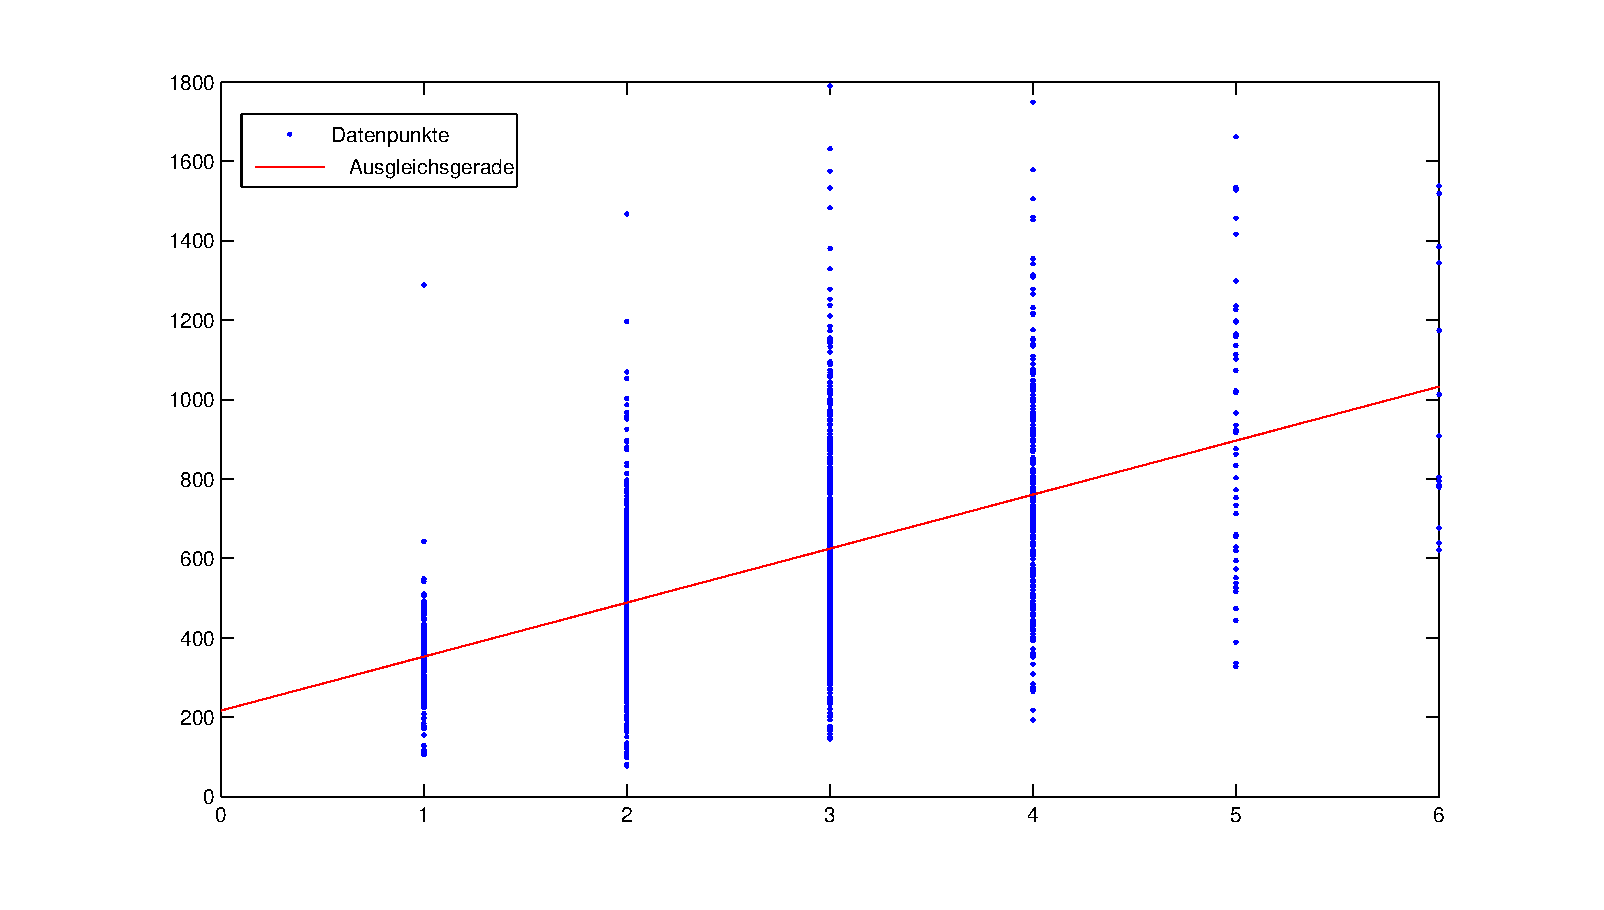
\includegraphics[width=0.8\textwidth]{figures/nm_rooms_distribution}
  \caption{Verteilung der Nettomieten in Abhängigkeit von der Raumanzahl mit der Berechneten Ausgleichsgeraden. Datensatz: Münchener Mietspiegel 2003 \cite{Fahrmeir2011}.}
  \label{fig:nm_rooms_distribution}
\end{figure}
Ziel der Regression ist es nun, den Mietpreis als Funktion der Raumanzahl darzustellen:
\begin{equation}
 M = f(R) + \epsilon
\end{equation}
, wobei $f$ eine beliebige Funktion und $\epsilon$ ein Fehlerterm ist.
Dieser wird benötigt, da die den Merkmalen zugehörigen Datensätze $(m_1, \dots, m_n)$, bzw. $(r_1, \dots, r_n)$ nie \textit{genau} auf der Regressionsgeraden liegen, sondern durch Messfehler oder nicht berücksichtigte Abhängigkeiten abweichen.
Der Erwartungswert für diese Fehler ist immer $0$. 
Um auch für kleinere Stichproben Aussagen über die Verteilung der Schätzer machen zu können, wird meinst zusätzlich eine normalverteilung angenommen \cite[S. 479]{Fahrmeir2010}:
% TODO: Notation der Normalverteilung hier erklären?
\begin{equation}
  E(\epsilon_i) = 0 \text{ und } \epsilon_i \sim N(0,\sigma^2), i = 1, \dots, n
\end{equation}

Diese Arbeit konzentriert sich nur auf lineare Funktionen $f$, aber in Abschnitt \ref{sec:mult_reg} wird gezeigt, wie auch ein logarithmischer Zusammenhang zwischen Regressand und Regressor miteinbezogen werden kann.
Hier ist aber ein linearer Zusammenhang naheliegend, daher wählen wir auch einen einfachen linearen Ansatz:
\begin{equation}
  M = \alpha + \beta R + \epsilon
\end{equation}
Dieser Ansatz lässt sich natürlich auf beliebige Merkmale übertragen.
Um nun die Ausgleichsgerade wie in Abbildung \ref{fig:nm_rooms_distribution} zu erhalten, ist es nötig die Parameter $\alpha$ und $\beta$ so zu schätzen, dass der quadratische Fehler minimal wird.
Dieses Verfahren wird  \textit{Methode der kleinsten Quadrate} genannt.
Formal sieht der Ansatz wie folgt aus:
\begin{equation}
  \sum\limits_{i=1}^{n} \epsilon^2 = \sum\limits_{i=1}^{n} (m_i - \alpha - \beta r_i)^2 \rightarrow \min\limits_{\alpha, \beta}
\end{equation}
Die minimierenden Werte werden mit $\hat\alpha$ und $\hat\beta$ notiert und als \textit{Kleinste-Quadrate-Schätzer} bezeichnet.
Für unseren linearen Ansatz können beide Schätzer relativ einfach berechnet werden.
Der Regressionskoeffizient $\hat\beta$ ist allgemein für zwei Merkmale $X$ und $Y$ gegeben durch
\begin{equation}
  \hat\beta = \frac{\tilde s_{XY}}{\tilde{s}^2_X} = \frac{\sum\limits_{i=1}^{n} y_i x_i - n \bar y \bar x}{\sum\limits_{i=1}^{n} x_i^2 - n \bar{x}^2}
\end{equation}
wobei $\tilde{s}^2_X$ die Varianz von $X$ und $\tilde s_{XY}$ die Kovarianz von $X$ und $Y$ bezeichnet. 
Wenn der Koeffizient bekannt ist, kann er in dir folgende Gleichnung eingesetzt werden um die Konstante $\alpha$ zu erhalten:
\begin{equation}
  \alpha = \bar y - \hat\beta \bar x
\end{equation}
Die Beweise für beide Rechnungen wurden hier aus Platzgründen ausgelassen, sind aber in \citet[S. 155]{Fahrmeir2010} zu finden.
% TODO: Muss der Durchschnitt hier erklärt werden?

Mithilfe dieser Methode erhalten wir nun die Schätzer für unser Beispiel.
Durch einfaches Einsetzen der Daten erhalten wir folgendes Ergebnis (Alle Zahlen wurden auf eine Stelle hinter dem Komma gerundet):
\begin{equation}
  \hat\beta = \frac{\sum\limits_{i=1}^{n} m_i r_i - n \bar m \bar r}{\sum\limits_{i=1}^{n} r_i^2 - n \bar{r}^2}
  = \frac{3309500 - 2053 * 570.1 * 2.6}{15833 - 2053 * 2.6^2}
  \approx 136
\end{equation}
\begin{equation}
  \hat\alpha = \bar m - \hat\beta \bar r 
  = 570.1 - 136 * 2.6 
  \approx 216.8
\end{equation}
Somit hat die Ausgleichsgerade in Abbildung \ref{fig:nm_rooms_distribution} die Gleichung $\hat m = 216.8 + 136 r$
Wir schreiben hier $\hat m$, da die Regressionsgerade eine Schäzung für die Nettomiete ist.

Die anfängliche Vermutung eines linearen Zusammenhangs zwischen der Anzahl der Zimmer und der Nettomiete ist damit bestätigt.
Man kann das Ergebnis weiterhin so interpretieren, dass es eine Grundmiete für jede Wohnung in Höhe von \EUR{216,80} für jede Wohnung gibt, die dann pro Zimmer um \EUR{136} erhöht wird.
Diese Interpretation ist allerdings in diesem Fall nicht unbedingt zielführend, da man schon mit bloßem Auge erkennen kann, dass die Residuen (Abweichungen der einzelnen Datenpunkte von der Ausgleichsgeraden) groß sind.
Daher wird die Annahme, wenn auch grundsätzlich richtig, wohl nur auf wenige Wohnungen zutreffen.
\\

Die Berechnung in der Funktion nag\_simple\_linear\_regression der \naglib erfolgt grundsätzlich wie oben beschrieben, allerdings mit einer Ausnahme: Es ist zusätzlich möglich die einzelnen Datenpunkte zu gewichten.
Dies führt dazu dass bei der Methode der kleinsten Quadrate auch die Fehler gewichtet eingehen, daher ist der Ansatz zur Minimierung dann $\sum\limits_{i=1}^{n}w_i\epsilon_i \rightarrow min$, wobei $w_i$ die Gewichtungen für die einzelnen Datenpunkte sind.
Für eine vollständige Beschreibung der Berechnungen mit Gewichtung sei der Leser auf \cite{nag:simple_regression} verwiesen.

% TODO: Vielleicht umbenennen in NAG Library Funktion oder so?
\subsubsection{Anwendung}
 
Nach der Beschreibung der Berechnung der einfachen linearen Regression wollen wir nun auf die Anwendung mittels der Funktion nag\_simple\_linear\_regression eingehen.
Die Funktionsdeklaration ist in Abbildung \ref{fig:nag_simple_linear} zu sehen.
\begin{figure}[t]
  \centering
\begin{lstlisting}
void nag_simple_linear_regression (Nag_SumSquare mean, 
     Integer n, const double x[], const double y[], 
     const double wt[], double *a, double *b, double *a_serr, 
     double *b_serr, double *rsq, double *rss, double *df,
     NagError *fail)
\end{lstlisting}
  \caption{Deklaration der Methode "nag\_simple\_linear\_regression", mit der eine einfache lineare Regression berechnet werden kann. }
  \label{fig:nag_simple_linear}
\end{figure}
Es existieren insgesamt 13 Parameter, von denen die ersten fünf Eingabe- und die Restlichen Ausgabeparameter sind.

Die wichtigsten Eingabeparameter sind die beobachteten Werte für das unabhängige(\lstinline{x[]}) und das abhängige(\lstinline{y[]}) Merkmal.
Für den Parameter \lstinline{n} muss nur die Anzahl der Beobachtungen angegeben und für \lstinline{wt[]} kann ein Array mit Gewichtungen für eingeragen werden.   
Falls keine Gewichtung gewünscht ist genügt es einen Null-Zeiger (zB. \lstinline{(double *) 0}) anzugeben.
Zuletzt existiert noch \lstinline{mean}.
Falls hier der Wert 'Nag\_AboutZero' angegeben wird, wird die Konstante $\alpha$ nicht in den Regressionsansatz miteinbezogen, d.h. die Regressionsgerade geht in jedem Fall durch den Ursprung.
Für die normale Berechnung kann 'Nag\_AboutMean' angegeben werden.

Die Ergebnisse der Regression $\hat\alpha$ und $\hat\beta$ sind nach Ausführung der Methode über die Zeiger \lstinline{*a} und \lstinline{*b} erreichbar.
Zudem werden auch einige Informationen zurückgegeben, die helfen die Güte des Regressionsansatzes zu überprüfen.
Da sind zunächst die Standardfehler \lstinline{*a_serr} und \lstinline{*b_serr}, die einen Hinweis darauf geben, wie genau die Koeffizienten geschätzt werden konnten.
Einen Hinweis auf die Güte des Regressionsmodells gibt das Bestimmtheitsmaß $R^2$ in \lstinline{*rsq}.
Es sagt aus, ein wie großer Anteil einer Variation des abhängigen Merkmals durch das unabhängige Merkmal erklärt wird.
Definiert ist es als Quadrat der Korrellation $R^2 = r_{XY}^2$ und nimmt daher Werte zwischen 0 und 1 an.
Ist der Wert niedrig, deutet dies auf ein schlechtes Regressionsmodell hin, da der Wert der abhängigen Variable dann stak von anderen, nicht beachteten, Einflüßen abhängig ist.
Zusätzlich wird noch die Summe der Fehlerquadrate (der minimierte Wert) in \lstinline{*rss} geschrieben.
Falls diese Summe sehr groß ist, weist das darauf hin, dass die Regressionsfunktion eine zu niedrige komplexität haben könnte, um den Zusammenhang zwischen Regressor und Regressand hinreichend abzubilden.

% TODO: Erwähnen, dass Beispielaufruf in Beispielprogramm verfügbar ist.

\begin{comment}
\begin{itemize}
 \item Nichtlineare Regression
 \begin{itemize}
  \item Für Sättigungskurven und Wachstumsverläufe
  \item Mögliche Funktionen: exp, $x^2$, sin
  \item Berechnung durch kleinste Quadrate Methode mittels Transformation möglich
 \end{itemize}

 \item Beispiel: Regression der Nettomiete nach Wohnfläche
 \begin{itemize}
  \item Streudiagramm zeigt steigende Abweichung $\Rightarrow$ Multiple Regression nötig!
 \end{itemize}
\end{itemize}

\subsubsection{Beispiel}


\end{comment}

\subsection{Multiple Regression}
\label{sec:mult_reg}

Im letzten Abschnitt haben wir behandelt, wie man mittels einfacher Regression die Werte eines abhängigen Merkmals auf Grundlage der Werte eines unabhängigen Merkmals schätzen kann.
Allerdings stößt die einfache Regression an Grenzen, wenn der Regressand von vielen Merkmalen beeinflußt wird, wobei die einzelnen Korrelationen an sich schwach sind.
Weiterhin bleiben offene Fragen: 
Wie verändert sich die Verteilung der Nettomieten zur Wohnungsfläche mit steigendem Baujahr?
Und wie groß ist der Einfluß von guter bzw. bester Wohnlage auf den Wohnungspreis? 

Für die Berechnung über Matrizen wird \cite{Fahrmeir1984} für die theoretischen Grundlagen verwendet.

Die multiple Regression ist zunächst einmal eine Erweiterung der einfachen Regression auf eine beliebige Anzahl von Regressoren.

\begin{equation}
  Y_i = \beta_0 + \beta_1 x_{i1} + \dots + \beta_p x_{ip} + \epsilon_i, \quad i = 1, \dots, n
\end{equation}
%TODO: Gleichung und Variablen erklären



\subsubsection{NAG Algorithmus}

In der NAG-Bibliothek wird die multiple Regression hauptsächlich durch die Funktion ... zur Verfügung gestellt.
%TODO: Welche anderen Funktionen sind noch beteiligt und was tuen diese?
 
%TODO: Ist eine alternative Strukturierung möglich, sodass weitere Unterkategorien wie QR-Zerlegung möglich sind?

\begin{equation}
  \label{eq:minimization}
  \sum\limits^{N}_{n=1} \epsilon^2_n = \epsilon^T \epsilon = (y - X \beta)^T (y - X \beta) \rightarrow \min\limits_{\beta}
\end{equation}


\begin{equation}
  \label{eq:minimization_general}
  \Vert X\beta - y \Vert_2 \rightarrow \min\limits_{\beta}
\end{equation}

\begin{equation}
  \label{eq:orthogonal_transformation}
  \Vert X\beta - y \Vert_2 = \Vert Q^T X \beta - Q^T y \Vert_2 = \Vert R \beta - c \Vert_2 + \Vert d \Vert_2
\end{equation}

\subsubsection{Anwendung}



\begin{figure}[t]
  \centering
\begin{lstlisting}
void nag_regsn_mult_linear (Nag_IncludeMean mean, Integer n, 
    const double x[], Integer tdx, Integer m, 
    const Integer sx[], Integer ip, const double y[], 
    const double wt[], double *rss, double *df, double b[], 
    double se[], double cov[], double res[], double h[], 
    double q[], Integer tdq, Nag_Boolean *svd, Integer *rank, 
    double p[], double tol, double com_ar[], NagError *fail)
\end{lstlisting}
  \caption{Deklaration der Methode nag\_regsn\_mult\_linear, welche eine multiple lineare Regressoin ausführt.}
  \label{fig:nag_multiple_linear}
\end{figure}

Zusatzlich zu nag\_regsn\_mult\_linear stellt die \naglib einige andere Funktionen zu Verfügung, die es ermöglichen das Regressionsmodell zu ändern, ohne die gesamte Regression erneut zu berechnen.
Diese Funktionen nehmen neben anderen Argumenten die QR-Zerlegung (welche von der Hauptfunktion als Zwischenergebnis ausgegeben wird), die zugehörigen Informationen welche im Parameter $p$ gespeichert wurden und die Beobachtungsmatrix $X$ und berechnen daraus aktualisierte Werte für die obere rechte Dreiecksmatrix $R$ und den Vektor $c$.
Im Gegensatz zu einer erneuten Berechnung mittels nag\_regsn\_mult\_linear hat dies den Vorteil, dass durch die Benutzung eines bereits bekannten Zwischenergebnisses Rechenzeit eingespart werden kann.
So kann der Benutzer beispielsweise mit nag\_regsn\_mult\_linear\_addrem\_obs neue Beobachtungen zum Modell hinzufügen oder sie entfernen.
Mittels nag\_regsn\_mult\_linear\_delete\_var und nag\_regsn\_mult\_linear\_add\_var werden aus dem Modell herausgenommen bzw. hinzugefügt, wobei die Beobachtungen im letzteren Fall schon in $X$ enthalten sein sollten.
Zusätzlich dazu ist es auch noch möglich die abhängige Variable zu tauschen (nag\_regsn\_mult\_linear\_newyvar).

Nach Anwendung dieser Funktionen können die neuen Regressionskoeffizienten $\beta_0, \beta_1, \dots$ durch einen Aufruf von nag\_regsn\_mult\_linear\_upd\_model unter Angabe von $R$ und $c$ erhalten werden.
Die einzelnen Funktionen werden in dieser Arbeit nicht einzelnd diskutiert, weitere Informationen sind aber unter \citep{nag:contents} verfügbar.

\begin{figure}[t]
  \centering
  \begin{narrow}{-0.2\textwidth}{0.2\textwidth}
    \subfloat[][Subfloat 1]{
      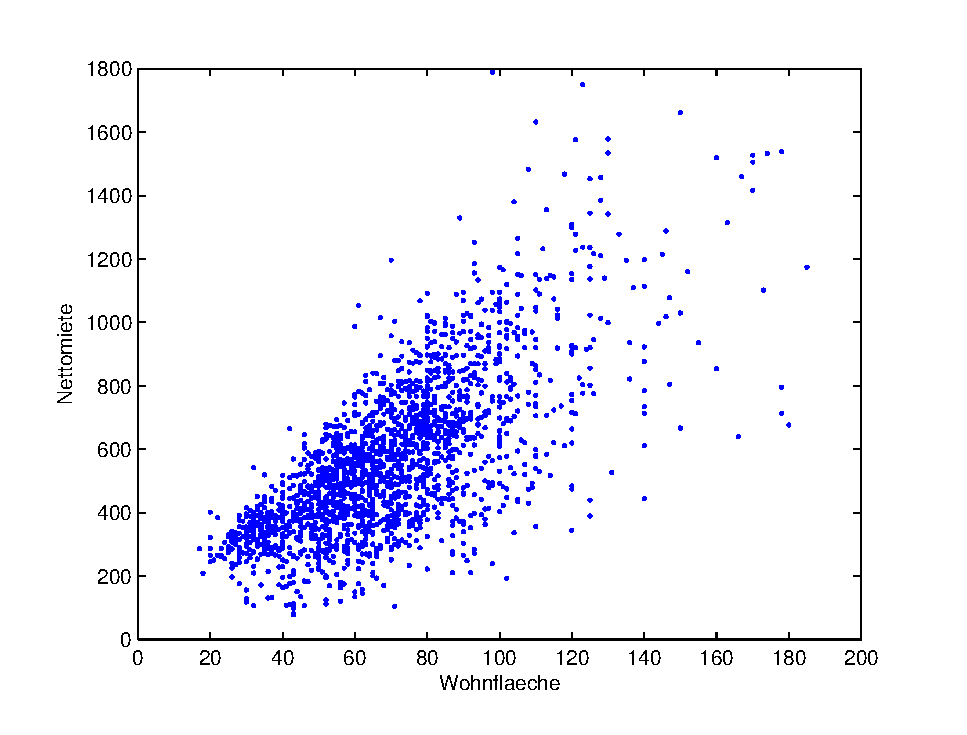
\includegraphics[width=0.7\textwidth]{figures/nm_wfl_distribution}
      \label{fig:nm_wfl_distributions:normal}
    }
    \subfloat[][Subfloat 2]{
      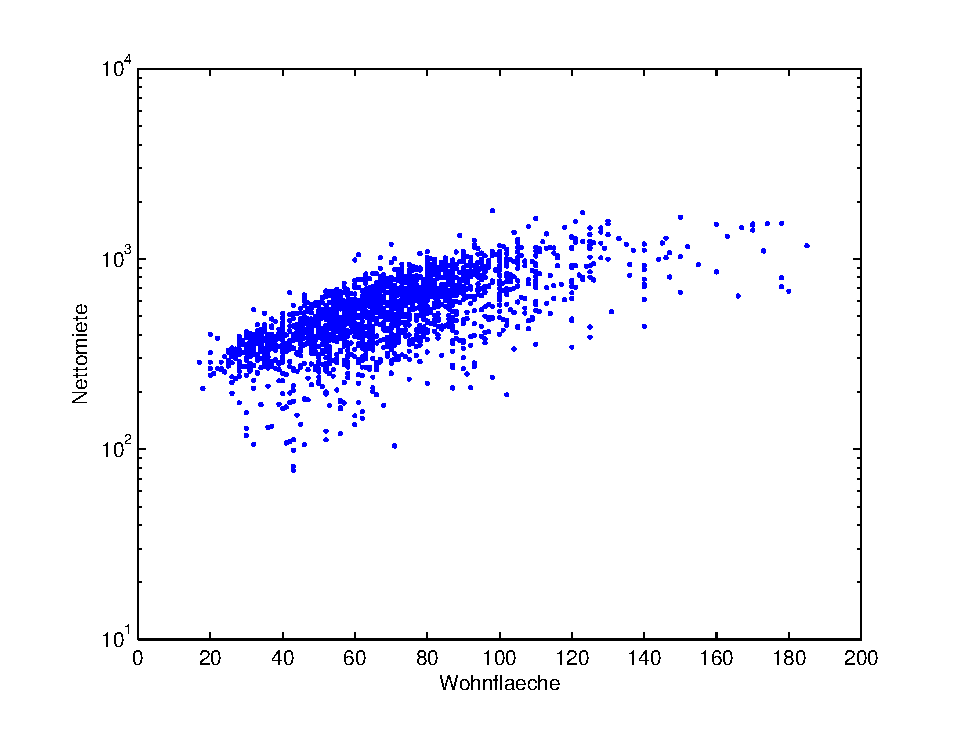
\includegraphics[width=0.7\textwidth]{figures/nm_wfl_distribution_log}
      \label{fig:nm_wfl_distributions:log}
    }
    \caption{Global caption}
  \end{narrow}
  \label{fig:nm_wfl_distributions}
\end{figure}

\begin{figure}[t]
  \centering
  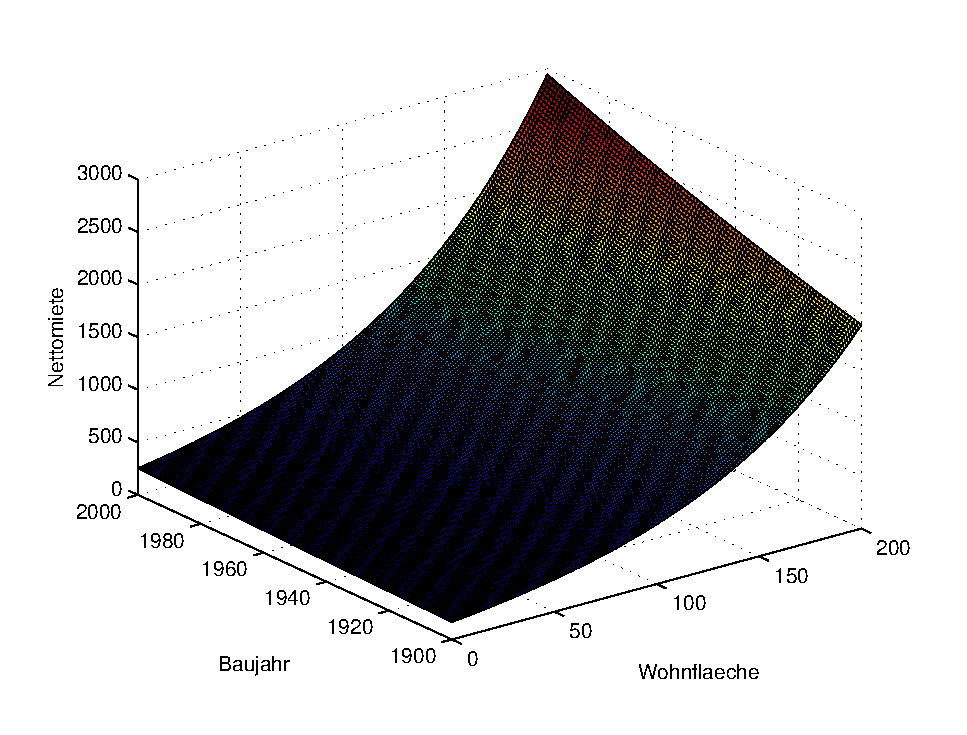
\includegraphics[width=10cm]{figures/nm_wfl_bj_log_approach}
  \caption{Caption}
  \label{fig:3d_result}
\end{figure}




%\subsection{Analyse}

%TODO:Überarbeiten oder herausnehmen!
%Zusätzlich zu der Berechnung der verschieden Regressionsmodelle bietet die {\it NAG C Library} auch Funktionen zur Auswahl des Regressionsmodells und zur Modellvalidierung.

%Für die Auswahl des Modells sollen in der Arbeit zwei Metriken behandelt werden: Die Residualstreuung und das Bestimmtheitsmaß $\mathcal{R}^2$.
%Beide können uns eine Idee davon geben, wie gut die unabhängigen Variablen die Werte der abhängigen Variablen erklären können.
%Die Residualstreuung gibt die Verteilung der Differenzen zwischen der angenäherten Funktion und den wirklichen Daten an.
%Sollte sie unregelmäßig sein (wenn die Residuen beispielsweise mit einer Variablen anwachsen) ist dies ein starkes Indiz dafür, dass ein zu simples Modell gewählt wurde. 
%Das Bestimmtheitsmaß gibt dagegen an, wie gut abhängige Variable durch die Regression erklärt werden kann.
%Berechnet werden kann es auch durch eine Quadrierung des Bravais-Pearson Korrelationskoeffizienten, was den starken Zusammenhang von Korrelation und Regressionsanalyse zeigt.

%Für die Modellvalidierung stehen verschiedene Werkzeuge zur Verfügung, welche bei der Bewertung der Güte der Regression und deren Verbesserung genutzt werden können.
%In diese Kategorie fallen zum Beispiel der Cooks-Abstand (ermittelt besonders einflußreiche Punkte), die T-Statistik (Testet, ob eine unabhängige Variable für die Regression wichtig ist) oder der Durbin-Watson-Test (Ermittelt, ob die Residuen von den zuvor gemessenen Werten abhängig sind.
%In dieser Arbeit werden diese allerdings nicht weiter behandelt werden.

%%% Local Variables: 
%%% mode: latex
%%% TeX-master: "report"
%%% End: 
